\documentclass[11pt,a4paper]{article}
\usepackage[utf8]{inputenc}
\usepackage{amsmath,amsfonts,amssymb}
\usepackage{graphicx}
\usepackage{geometry}
\geometry{margin=1in}
\usepackage{booktabs}
\usepackage{hyperref}
\usepackage{float}
\usepackage{xcolor}

\title{\textbf{EE3621: Digital Signal Processing} \\ \Large Lecture 9: Fast Fourier Transform (FFT) --- Decimation in Time (DIT) \\ \large (III B.Tech EEE)}
\author{Lecture Notes (40-Minute Plan)}
\date{}

\definecolor{darkbg}{HTML}{0d121f}
\definecolor{lighttext}{HTML}{e2e8f0}
\definecolor{primary}{HTML}{8b5cf6}
\definecolor{secondary}{HTML}{0dd5c5}

\pagecolor{darkbg}
\color{lighttext}

\hypersetup{
    colorlinks=true,
    linkcolor=secondary,
    urlcolor=secondary
}

\begin{document}

\maketitle

\section{Lecture Plan (40 Minutes Breakdown)}
\begin{itemize}
    \item \textbf{00:00 -- 05:00 (5 mins):} Welcome, Unit II Intro. The problem with Direct DFT --- Computational Complexity Motivation.
    \item \textbf{05:00 -- 15:00 (10 mins):} The core idea of FFT: Divide and Conquer strategy. Decimating the time-domain signal into even and odd indices.
    \item \textbf{15:00 -- 20:00 (5 mins):} Twiddle factor mathematics and reduction proofs.
    \item \textbf{20:00 -- 25:00 (5 mins):} The 2-point Butterfly operation. Understanding the basic building block.
    \item \textbf{25:00 -- 30:00 (5 mins):} Signal Flow Graph for $N=8$, Bit-Reversal permutation, and intuitive understanding.
    \item \textbf{30:00 -- 35:00 (5 mins):} Complexity Analysis and Comparison Table. Implementing IFFT via FFT.
    \item \textbf{35:00 -- 40:00 (5 mins):} Checkpoint questions with detailed answers and conclusion.
\end{itemize}

\noindent\rule{\textwidth}{0.5pt}

\section{Computational Complexity Motivation}

\begin{figure}[H]
    \centering
    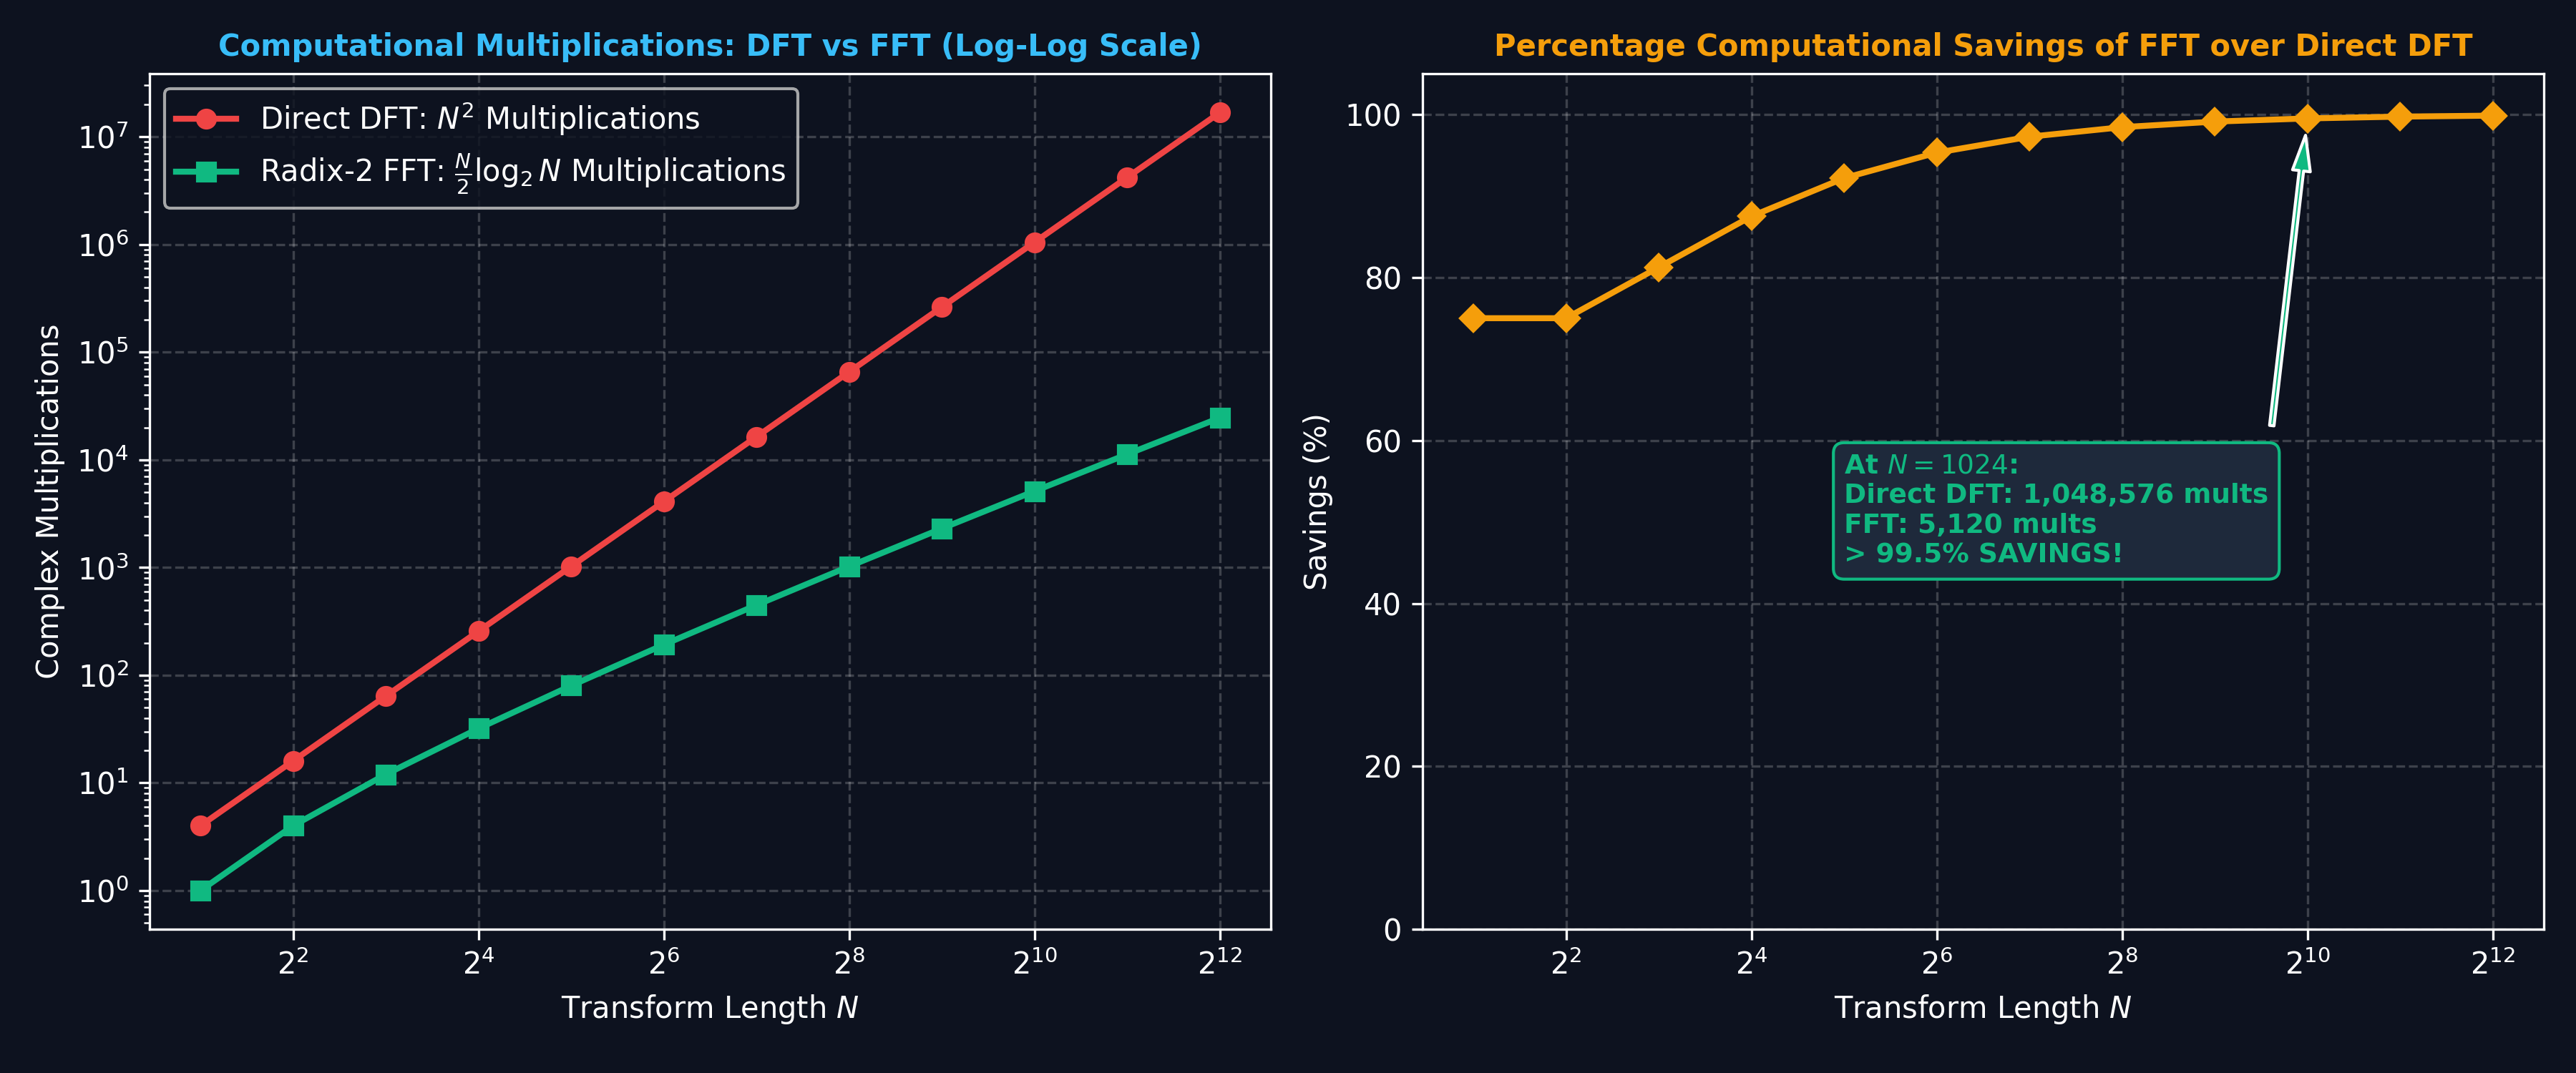
\includegraphics[width=0.85\textwidth]{images/dft_vs_fft_complexity.png}
    \caption{Computational Scaling: Direct DFT $O(N^2)$ vs. Radix-2 FFT $O(N \log_2 N)$ ($>99.5\%$ Savings for $N=1024$).}
\end{figure}

\begin{figure}[H]
    \centering
    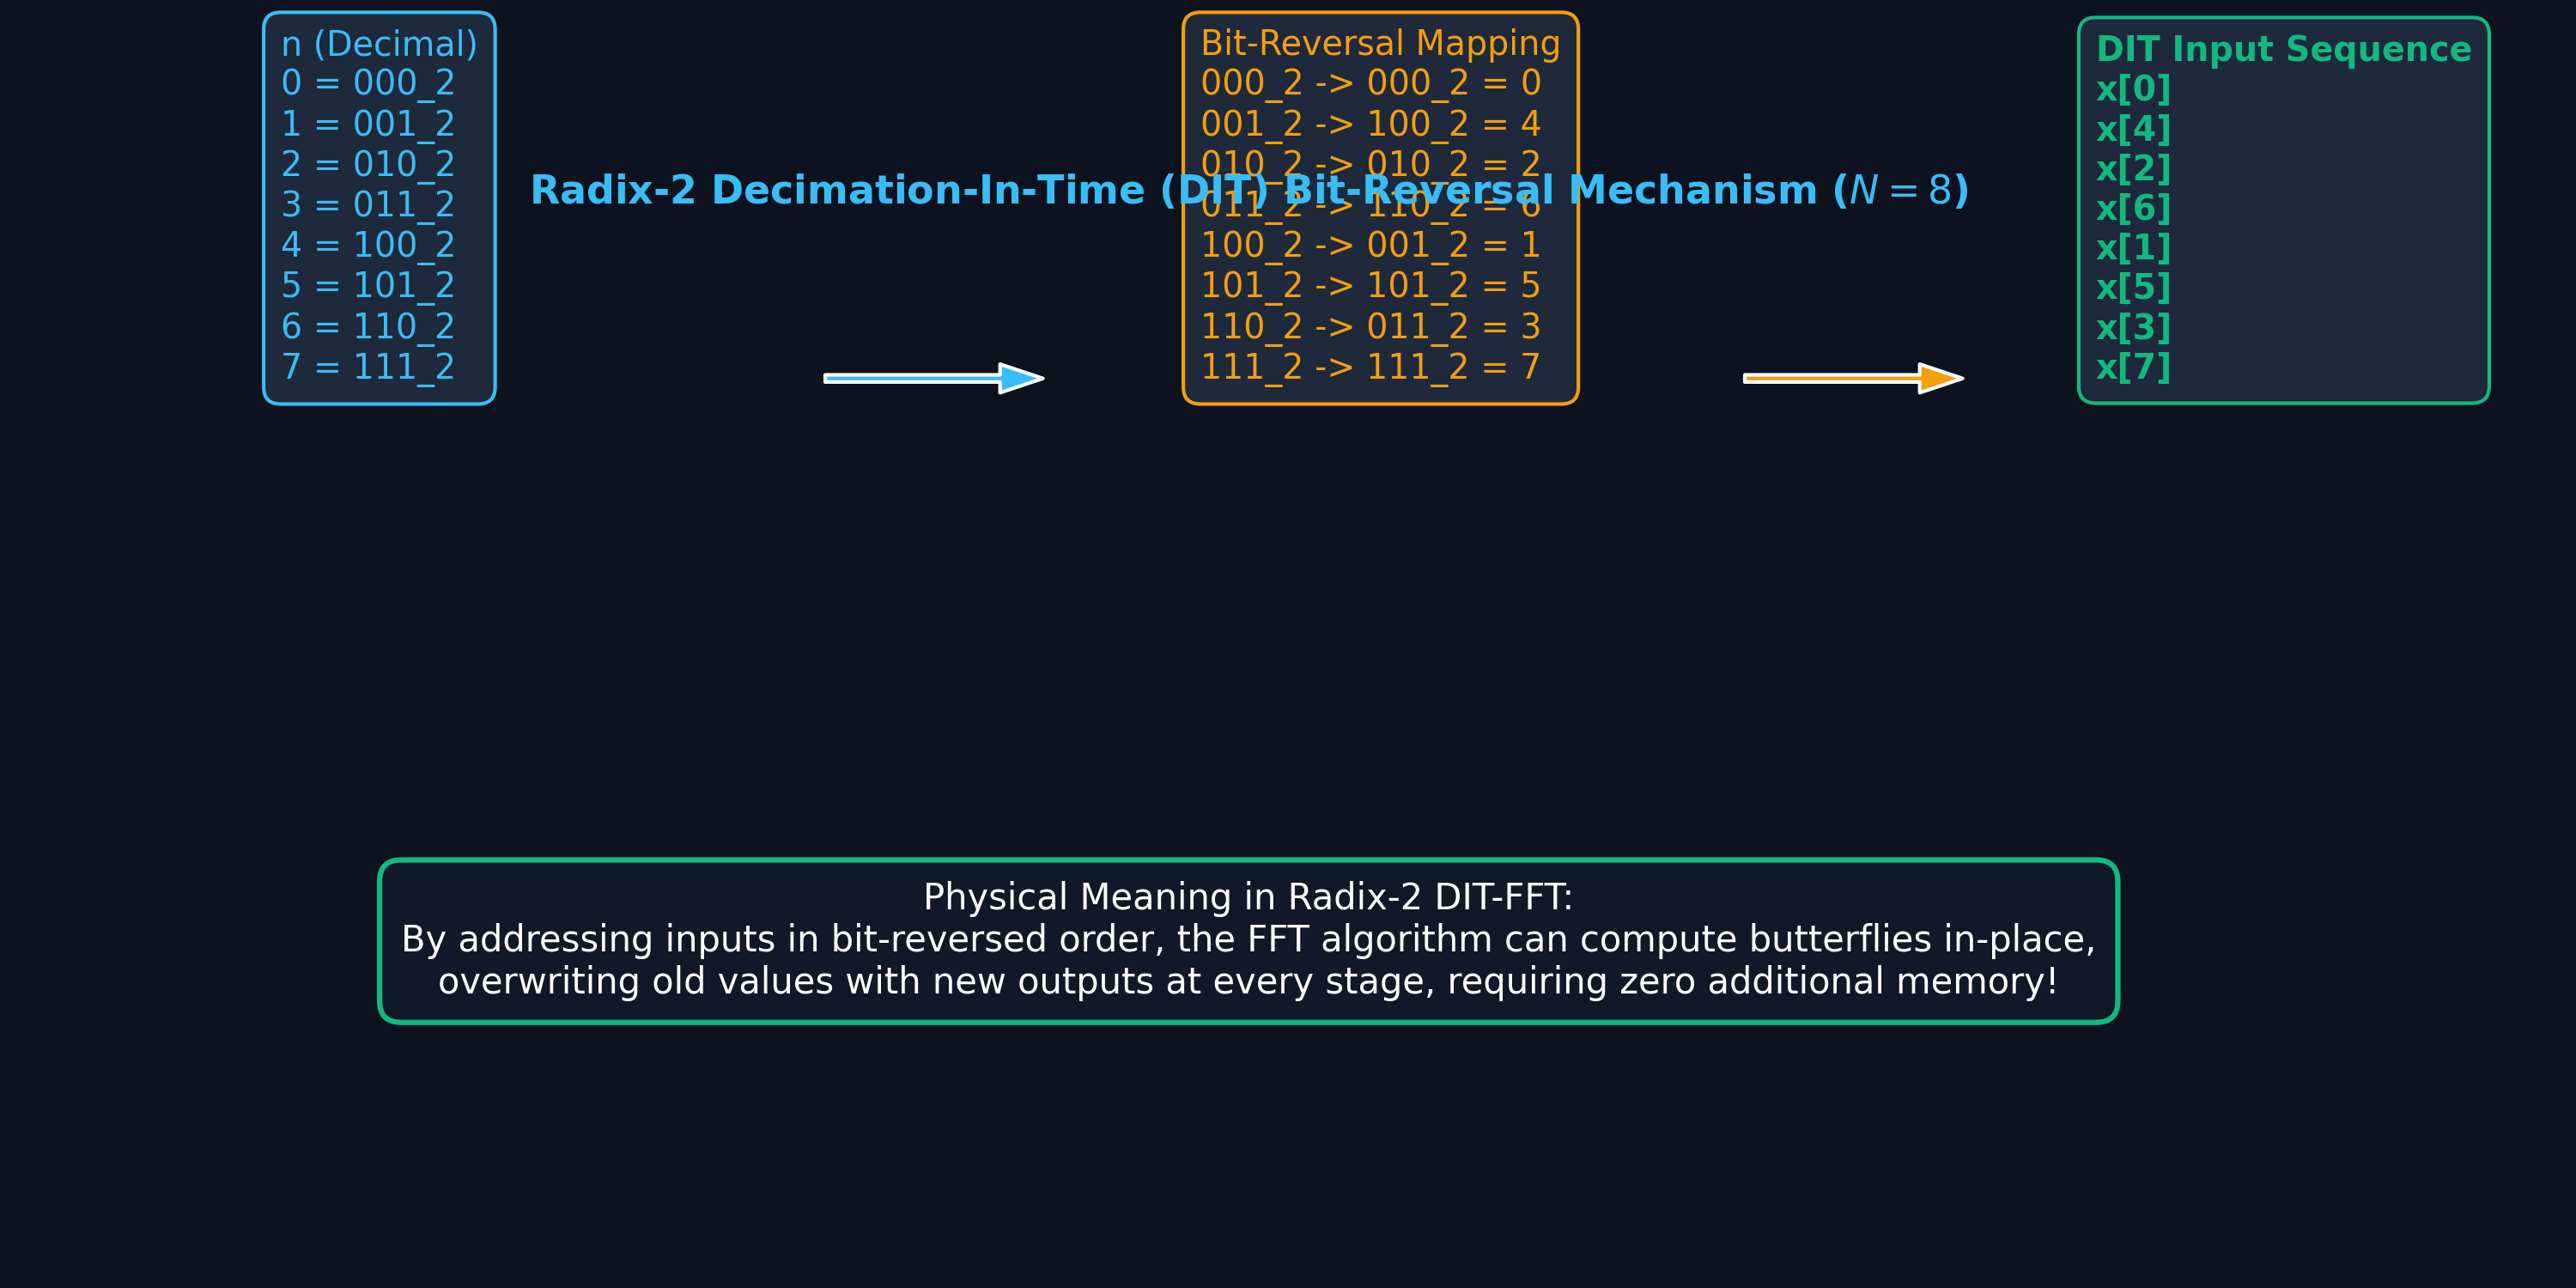
\includegraphics[width=0.85\textwidth]{images/dit_bit_reversal_tree.png}
    \caption{Radix-2 Decimation-in-Time Bit-Reversal Address Mapping for In-Place Memory Execution.}
\end{figure}

\begin{figure}[H]
    \centering
    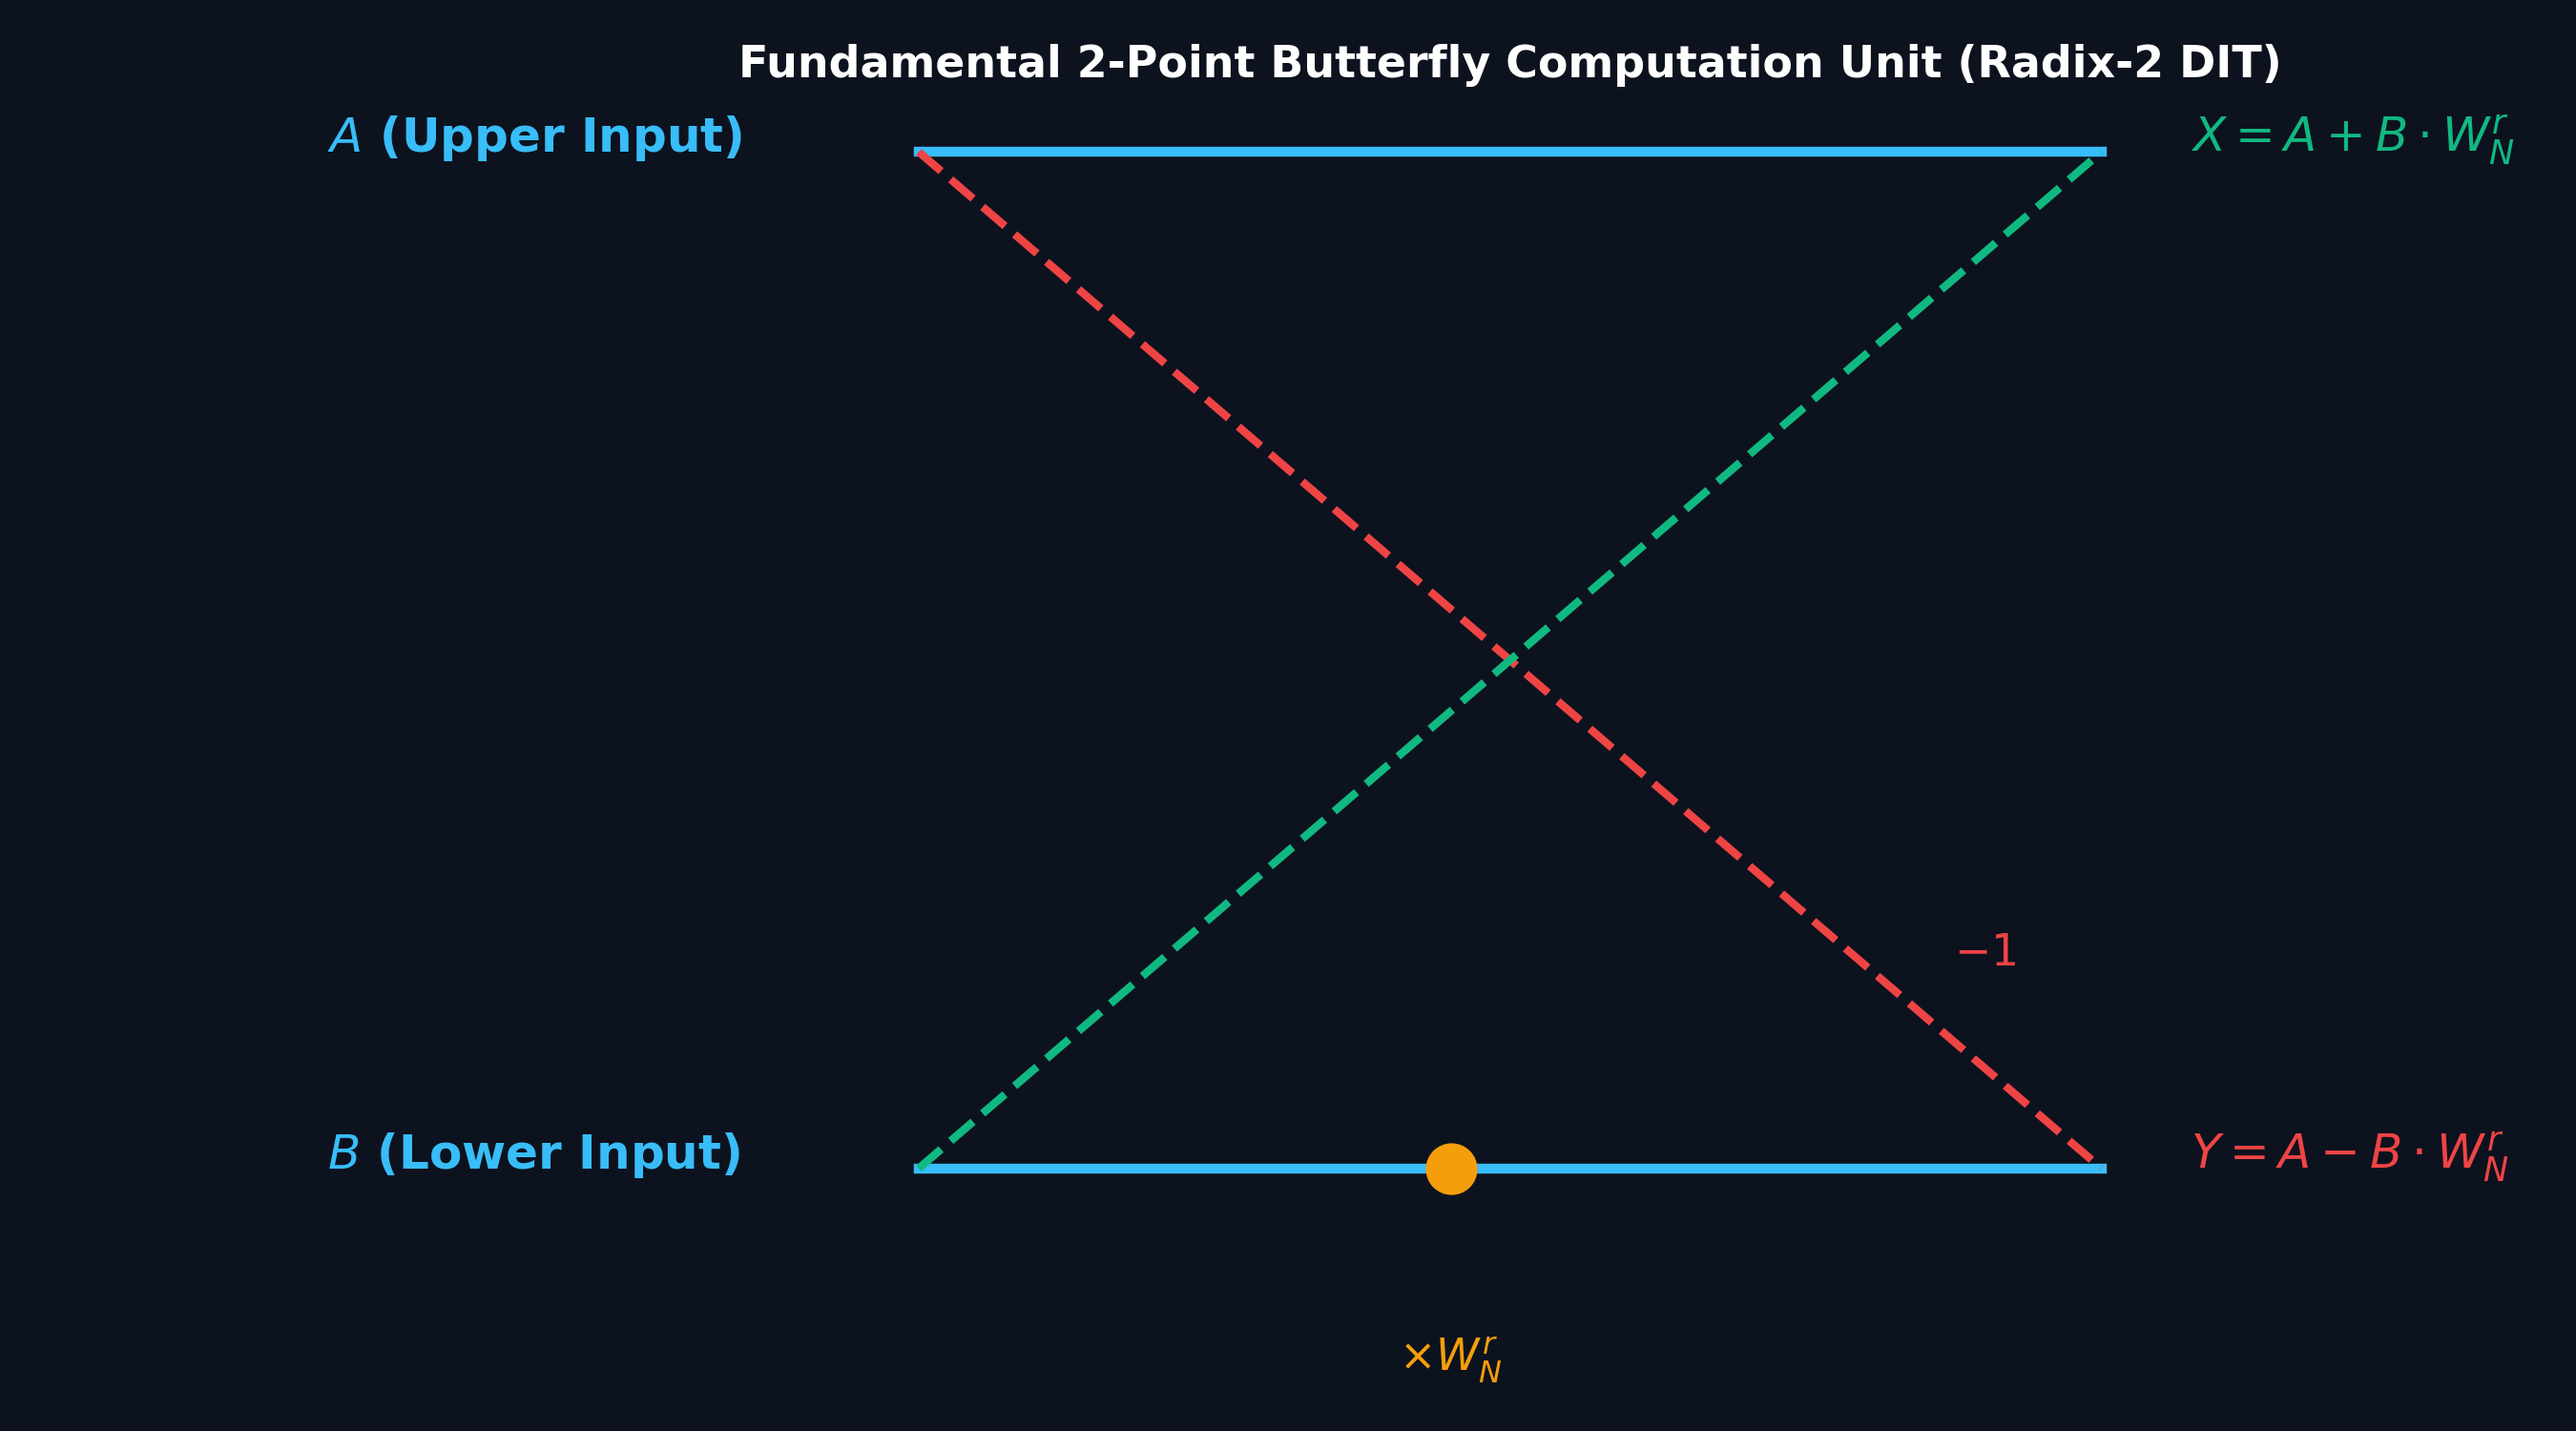
\includegraphics[width=0.75\textwidth]{images/fft_butterfly.png}
    \caption{Fundamental 2-Point Butterfly Computation Unit (Radix-2 DIT).}
\end{figure}


The Direct Discrete Fourier Transform (DFT) of an $N$-point sequence $x[n]$ is given by:
\begin{equation}
X[k] = \sum_{n=0}^{N-1} x[n] W_N^{kn}
\end{equation}
where $W_N = e^{-j \frac{2\pi}{N}}$ is the twiddle factor, and $0 \le k \le N-1$.

Let's carefully count the operations for the direct calculation:
\begin{enumerate}
    \item For each frequency bin $X[k]$, we must multiply $N$ complex numbers $x[n]$ by $N$ complex twiddle factors $W_N^{kn}$. This requires $N$ complex multiplications.
    \item Summing these $N$ terms requires $N-1$ complex additions.
    \item Since there are $N$ frequency bins (from $k=0$ to $N-1$), the total operations are:
    \begin{itemize}
        \item \textbf{Total Complex Multiplications:} $N \times N = N^2$
        \item \textbf{Total Complex Additions:} $N \times (N-1) = N^2 - N$
    \end{itemize}
\end{enumerate}

For small $N$, this is fine. But consider a typical audio block of $N=1024$:
Number of complex multiplications = $1024^2 = 1,048,576 > 10^6$. Since one complex multiplication requires 4 real multiplications and 2 real additions, the burden is massive. Real-time processing becomes impossible for longer sequences without a better algorithm.

The Fast Fourier Transform (FFT) reduces this complexity from $O(N^2)$ to $O(N \log_2 N)$. For $N=1024$, the FFT requires only $\frac{N}{2}\log_2 N = 512 \times 10 = 5120$ multiplications.

\section{Divide \& Conquer Decomposition: Decimation in Time (DIT)}
The Radix-2 DIT FFT algorithm works by recursively dividing an $N$-point sequence (where $N$ is a power of 2) into two shorter sequences of length $N/2$. 

Let us separate $x[n]$ into its even-indexed and odd-indexed samples:
\begin{itemize}
    \item Even samples: $x_e[m] = x[2m]$ for $m = 0, 1, \dots, \frac{N}{2}-1$
    \item Odd samples: $x_o[m] = x[2m+1]$ for $m = 0, 1, \dots, \frac{N}{2}-1$
\end{itemize}

Substitute this into the DFT equation:
\begin{equation}
X[k] = \sum_{m=0}^{N/2-1} x[2m] W_N^{2mk} + \sum_{m=0}^{N/2-1} x[2m+1] W_N^{(2m+1)k}
\end{equation}

Factor out $W_N^k$ from the second summation:
\begin{equation}
X[k] = \sum_{m=0}^{N/2-1} x[2m] W_N^{2mk} + W_N^k \sum_{m=0}^{N/2-1} x[2m+1] W_N^{2mk}
\end{equation}
This is the foundational equation of the DIT FFT!

\section{Twiddle Factor Reduction}
\textbf{Theorem:} $W_N^2 = W_{N/2}$ \\
\textbf{Proof:}
\begin{align*}
W_N^2 &= \left( e^{-j \frac{2\pi}{N}} \right)^2 \\
W_N^2 &= e^{-j \frac{4\pi}{N}} \\
W_N^2 &= e^{-j \frac{2\pi}{N/2}} \\
W_N^2 &= W_{N/2}
\end{align*}

Applying this identity: $W_N^{2mk} = (W_N^2)^{mk} = W_{N/2}^{mk}$, we rewrite our split DFT equation:
\begin{equation}
X[k] = \sum_{m=0}^{N/2-1} x_e[m] W_{N/2}^{mk} + W_N^k \sum_{m=0}^{N/2-1} x_o[m] W_{N/2}^{mk}
\end{equation}

The first sum is the $N/2$-point DFT of the even sequence, $G[k]$. The second sum is the $N/2$-point DFT of the odd sequence, $H[k]$.
\begin{equation}
\textbf{KEY RESULT: } X[k] = G[k] + W_N^k H[k]
\end{equation}

For the upper half of the spectrum ($k \ge N/2$), we use the symmetry property $W_N^{k+N/2} = -W_N^k$:
\begin{equation}
X[k+N/2] = G[k] - W_N^k H[k]
\end{equation}

\section{The Butterfly Operation}
The equations:
\begin{align}
X[k] &= G[k] + W_N^k H[k] \\
X[k+N/2] &= G[k] - W_N^k H[k]
\end{align}
form the \textbf{Butterfly Operation}. If we let $A = G[k]$ and $B = H[k]$, the outputs $A'$ and $B'$ are:
\begin{align}
A' &= A + W_N^k B \\
B' &= A - W_N^k B
\end{align}
\textbf{Engineering Intuition:} Instead of multiplying $B$ by $W_N^k$ and separately by $-W_N^k$, we calculate $(W_N^k B)$ once, add it to $A$, and subtract it from $A$. This halves multiplications.

\section{Signal Flow Graph \& Bit-Reversal Permutation}
For $N=8$, the sequence is recursively divided until 2-point DFTs are reached. The final input order is: $x[0], x[4], x[2], x[6], x[1], x[5], x[3], x[7]$.

\textbf{Why this order?} Observe the binary index:
\begin{itemize}
    \item $1 \rightarrow 001 \rightarrow$ reversed: $100 \rightarrow 4$
    \item $2 \rightarrow 010 \rightarrow$ reversed: $010 \rightarrow 2$
    \item $3 \rightarrow 011 \rightarrow$ reversed: $110 \rightarrow 6$
\end{itemize}
This is the \textbf{Bit-Reversal Permutation}.

\subsection{The 8-Point DIT-FFT Stages}
\begin{itemize}
    \item \textbf{Stage 1:} Four 2-point butterflies.
    \item \textbf{Stage 2:} Two 4-point FFT blocks using $W_8^0$ and $W_8^2$.
    \item \textbf{Stage 3:} One 8-point FFT block using $W_8^0, W_8^1, W_8^2, W_8^3$.
\end{itemize}

\section{Complexity Analysis}
Let $T(N)$ be the number of complex multiplications for an $N$-point FFT.
An $N$-point DFT requires:
\begin{enumerate}
    \item Two $N/2$-point DFTs: $2 T(N/2)$
    \item $N/2$ multiplications by $W_N^k$ for the butterflies.
\end{enumerate}
Recurrence relation:
\begin{equation}
T(N) = 2T(N/2) + \frac{N}{2}
\end{equation}
\textbf{Proof by Recursion:}
\begin{align*}
T(N) &= 2 \left( 2T(N/4) + \frac{N}{4} \right) + \frac{N}{2} = 4T(N/4) + 2\frac{N}{2}
\end{align*}
After $\nu = \log_2 N$ stages, we reach $T(1) = 0$:
\begin{equation}
T(N) = 2^{\nu}T(N/2^{\nu}) + \nu \frac{N}{2} = \frac{N}{2}\log_2 N
\end{equation}

\section{Comparison Table: DFT vs FFT}
\begin{table}[H]
\centering
\begin{tabular}{@{}llll@{}}
\toprule
\textbf{Signal Length $N$} & \textbf{Direct Multiplications} & \textbf{FFT Multiplications} & \textbf{Speedup Factor} \\ \midrule
8 & 64 & 12 & 5.3x \\
64 & 4,096 & 192 & 21.3x \\
256 & 65,536 & 1,024 & 64.0x \\
1024 & 1,048,576 & 5,120 & 204.8x \\
4096 & 16,777,216 & 24,576 & 682.7x \\ \bottomrule
\end{tabular}
\caption{Complexity comparison}
\end{table}

\section{Computing IFFT using FFT}
The Inverse DFT (IDFT) is:
\begin{equation}
x[n] = \frac{1}{N} \sum_{k=0}^{N-1} X[k] W_N^{-kn}
\end{equation}
Using the \textbf{conjugate trick}, take the complex conjugate of $x[n]$:
\begin{equation}
x^*[n] = \frac{1}{N} \sum_{k=0}^{N-1} X^*[k] W_N^{kn} = \frac{1}{N} \text{FFT}\{X^*[k]\}
\end{equation}
Taking the conjugate again:
\begin{equation}
x[n] = \frac{1}{N} \left( \text{FFT}\{X^*[k]\} \right)^*
\end{equation}
\textbf{Physical Intuition:} Conjugate the frequency data, run forward FFT, conjugate output, and divide by $N$.

\section{Checkpoint Questions}
\textbf{Q1: In an 8-point Radix-2 DIT FFT, what is the index for the 5th element?} \\
\textbf{Answer:} Normal index 4 $\rightarrow$ binary $100_2 \rightarrow$ reverse $001_2 \rightarrow$ decimal 1. It is $x[1]$.

\vspace{10pt}
\noindent
\textbf{Q2: At 20 ns per complex multiplication, calculate time saved by FFT for $N=4096$.} \\
\textbf{Answer:} 
\begin{itemize}
    \item Direct: $4096^2 \times 20$ ns = 335.54 ms
    \item FFT: $24576 \times 20$ ns = 0.491 ms
    \item Saved: $\sim$335.05 ms.
\end{itemize}

\vspace{10pt}
\noindent
\textbf{Q3: Prove $W_N^{k+N/2} = -W_N^k$ and its use.} \\
\textbf{Answer:} 
$W_N^{k+N/2} = W_N^k \cdot W_N^{N/2} = W_N^k \cdot e^{-j\pi} = -W_N^k$. Used in the butterfly operation to reduce multiplications by sharing terms.

\section{Table of Key Formulas}
\begin{table}[H]
\centering
\begin{tabular}{@{}ll@{}}
\toprule
\textbf{Concept} & \textbf{Formula / Property} \\ \midrule
Direct DFT & $X[k] = \sum_{n=0}^{N-1} x[n] W_N^{kn}$ \\
Twiddle Factor & $W_N = e^{-j \frac{2\pi}{N}}$ \\
Symmetry Property & $W_N^{k + N/2} = -W_N^k$ \\
Periodicity Property & $W_N^{k + N} = W_N^k$ \\
Square Property & $W_N^2 = W_{N/2}$ \\
DIT Decomposition & $X[k] = G[k] + W_N^k H[k]$ \\
FFT Multiplications & $\frac{N}{2}\log_2 N$ \\
IFFT via FFT & $x[n] = \frac{1}{N} ( \text{FFT}\{X^*[k]\} )^*$ \\ \bottomrule
\end{tabular}
\end{table}

\end{document}
